\chapter{Experimentos y validación}
\label{chap:experimentos}

El objetivo de este capítulo es mostrar el funcionamiento de la aplicación en un caso de uso real en el que se tratará de extraer conclusiones generales acerca del consumo eléctrico de cada modelo y de si este consumo irá necesariamente acompañado de una mejora de los resultados de predicción.
Para ello se emplearán las herramientas descritas anteriormente para evaluar el consumo y el rendimiento de una serie de modelos formada por representantes de las principales familias de modelos de aprendizaje automático y recogidos en la sección~\ref{sec:models}. Estos modelos serán aplicados a los conjuntos de datos de distintas características definidos en la sección~\ref{sec:datasets}.

\section{Estructura de los experimentos}

Durante la validación de la aplicación se llevarán acabo dos experimentos distintos.
El primero examinará el consumo energético en base al modelo seleccionado. En esta sección se tomarán varias medidas de consumo y rendimiento por modelo y conjunto de datos en una máquina con unos recursos de procesamiento concretos para analizar que modelos consumen más que otros y que características de los conjuntos de datos hacen incrementar este consumo.
El segundo experimento seleccionará un único conjuntos de datos de tamaño mediano y tomará medidas de consumo en tres entornos con distintos recursos de procesamiento dedicados a la tarea de aprendizaje automático para observar el efecto de los recursos disponibles en el consumo energético de cada modelo.

A través de este análisis, se pretende obtener una comprensión profunda de cómo diferentes modelos de aprendizaje automático consumen energía bajo diversas condiciones de trabajo. Además se intentarán identificar patrones de menor consumo que puedan utilizarse como base para el diseño y la implementación de modelos más sostenibles y eficientes en el futuro.


\begin{figure}[H]
  \centerline{
     
\includegraphics[width=0.8\textwidth, keepaspectratio]{img/placeholder.png}
  }
  \caption{Esquema general a seguir durante los experimentos}
  \label{fig:esquema-experimentos}
\end{figure}
\todo[inline]{Añadir esquema}

\section{Consumo energético en función del modelo seleccionado}
\label{sec:test-1-models}

\subsubsection{Objetivos}

En esta sección se examinará el consumo energético una serie de modelos representativos aplicados a varios conjuntos de datos. El objetivo de este análisis será abordar las siguientes cuestiones clave:

\begin{itemize}
    \item Identificación de los modelos con mayor consumo energético.
    \item Determinación de los modelos cuyo consumo energético incrementa significativamente al aumentar el número de muestras.
    \item Evaluación de modelos que ofrecen mejores predicciones con menor consumo energético.
\end{itemize}

Dónde sea posible, se tratará de analizar estas cuestiones de forma general y obtener conclusiones que sean extrapolables más allá de los conjuntos de datos concretos que se hayan medido. Sin embargo, debido a la gran cantidad de variables involucradas en las variaciones de consumo entre unos casos y otros, es posible en otros conjuntos de datos se observen comportamientos distintos del consumo.

\subsubsection{Metodología}

Para analizar estas cuestiones todas las medidas de consumo serán tomadas con la aplicación desarrollada ejecutando en una misma máquina. Para cada modelo y conjunto de datos, se tomarán medidas de consumo y rendimiento utilizando validación cruzada con cinco iteraciones con un tamaño definido para los datos de testeo del 20\% del conjunto de datos. Esta técnica proporcionará una evaluación robusta y precisa tanto del comportamiento energético de los modelos como de su precisión y exactitud, ya que evitará en gran medida la presencia de valores atípicos y el riesgo de sobreajuste de los modelos.

\begin{table}[h]
    \caption{Características técnicas de la máquina utilizada para tomar las medidas}
    \label{tab:caracteristicas-tecnicas}
    \renewcommand\arraystretch{1.4}
    \centering
    \begin{tabular}{m{0.3\textwidth} m{0.55\textwidth}}
        \toprule
         \textbf{Característica} & \textbf{Descripción} \\
         \midrule
         Modelo & Dell XPS 15 9500\\
         Sistema Operativo & Ubuntu 20.04.6 LTS x86\_64\\
         Procesador & Intel(R) Core(TM) i9-10885H CPU @ 2.40GHz\\
         Versión Python & 3.12.2\\
         Memoria & 7,63 GB\\
         \bottomrule
    \end{tabular}
\end{table}

La aplicación será ejecutada con el siguiente comando para cada conjunto de datos distinto, en el cual \texttt{[dataset]} será sustituido por el archivo que contenga cada conjunto de datos. Adicionalmente, cualquiera de las opciones de lectura de datos descritas en la sección~\ref{sec:limpieza} podrá ser utilizada si el formato en el que se encuentren los datos lo requiere. Las características de la máquina utilizada están recogidas en la tabla~\ref{tab:caracteristicas-tecnicas}.
\begin{minted}{bash}
mlcost measure --log -cv 5 -d [dataset] [dataset-options]
\end{minted}

\subsubsection{Resultados}

La ejecución del comando anterior producirá un archivo tipo tabla de datos en formato \texttt{.csv}. La tabla~\ref{tab:medidas-1} recoge un extracto de los resultados obtenidos en el ordenador de referencia para seis conjuntos de datos distintos. El archivo completo está disponible en el repositorio de la aplicación.

\begin{table}[H]
\caption[Extracto de los resultados de entrenamiento]{Extracto de los resultados de entrenamiento\footnote{\url{https://github.com/l-gonz/tfg-gitt-mlcost/blob/main/model-comp-many.csv}}.}

\label{tab:medidas-1}
\renewcommand\arraystretch{1.4}
\centerline{
\scalebox{0.75}{
\begin{tabular}{ >{\raggedright\arraybackslash}p{0.11\textwidth}  % Name
                 >{\raggedright\arraybackslash}p{0.1\textwidth}  % Model
                 >{\raggedleft\arraybackslash}p{0.11\textwidth} % CPU Load
                 >{\raggedleft\arraybackslash}p{0.11\textwidth}  % Acc
                 >{\raggedleft\arraybackslash}p{0.11\textwidth}  % Prec
                 >{\raggedleft\arraybackslash}p{0.09\textwidth}  % F-score
                 >{\raggedleft\arraybackslash}p{0.08\textwidth} % Recall
                 >{\raggedleft\arraybackslash}p{0.09\textwidth}  % Fit
                 >{\raggedleft\arraybackslash}p{0.07\textwidth} % Time
                 >{\raggedleft\arraybackslash}p{0.12\textwidth} % Emiss
                 >{\raggedleft\arraybackslash}p{0.1\textwidth}  % Ener
                 >{\raggedleft\arraybackslash}p{0.05\textwidth} % Samples
                 }
\toprule
\textbf{Dataset}     & \textbf{Modelo} & \textbf{CPU load (\%)} & \textbf{Accuracy} & \textbf{Precision} & \textbf{F-score} & \textbf{Recall} & \textbf{Fit time (s)}  & \textbf{Total (s)} & \textbf{Emisiones (kg)} & \textbf{Energía (kWh)}  & \textbf{N} \\ 
\midrule
Banknote    & Linear & 2.7     & 0.98    & 0.98  & 0.98 & 0.98 & 0.007             & 0.071 & 2.13E-07 & 1.10E-06 & 1372 \\
Banknote    & Linear & 2.7      & 0.97  & 0.97  & 0.97  & 0.97  & 0.006             & 0.071       & 2.13E-07  & 1.10E-06 & 1372     \\
Banknote    & Linear & 2.7     & 0.97      & 0.97      & 0.97    & 0.97 & 0.006             & 0.071      & 2.13E-07  & 1.10E-06 & 1372     \\
Banknote    & Linear & 2.7     & 0.99      & 0.99   & 0.99  & 0.99  & 0.005             & 0.071      & 2.13E-07  & 1.10E-06 & 1372     \\
Banknote    & Linear & 2.7     & 0.99      & 0.99      & 0.99 & 0.99  & 0.005             & 0.071      & 2.13E-07  & 1.10E-06 & 1372     \\
Banknote    & Forest & 2.7      & 0.99      & 0.99      & 0.99    & 0.99  & 0.184             & 1.429     & 3.27E-06  & 1.69E-05 & 1372     \\
Banknote    & Forest & 2.7    & 1.00  & 1.00      & 1.00    & 1.00   & 0.171             & 1.429  & 3.27E-06  & 1.69E-05 & 1372     \\
Banknote    & Forest & 2.7   & 0.99   & 0.99      & 0.99    & 0.99 & 0.154             & 1.429  & 3.27E-06  & 1.69E-05 & 1372     \\
Banknote    & Forest & 2.7   & 1.00   & 1.00      & 1.00    & 1.00  & 0.172             & 1.429  & 3.27E-06  & 1.69E-05 & 1372     \\
Banknote    & Forest & 2.7    & 1.00  & 1.00      & 1.00    & 1.00  & 0.158             & 1.429    & 3.27E-06  & 1.69E-05 & 1372     \\
\multicolumn{12}{ c }{$\dots$} \\
Electricity & Neural & 102.4         & 0.82      & 0.83      & 0.83    & 0.83          & 132.768           & 518.905          & 1.19E-03  & 6.15E-03 & 45312 \\
\bottomrule
\end{tabular}}}
\end{table}

Cada fila en la tabla corresponde a las medidas tomadas durante una iteración de entrenamiento de cada modelo por validación cruzada. Al haber escogido utilizar validación cruzada de cinco iteraciones, la tabla de resultados cuenta con cinco filas por modelo y conjunto de datos. Sin embargo, algunas de las medidas, como la carga del procesador, el número de muestras del conjunto de datos, el tiempo total de entrenamiento, las emisiones del proceso y la energía consumida, son tomadas de forma global al finalizar todas las iteraciones de entrenamiento de cada modelo y conjunto.
Para cada iteración individual se recogen las medidas estadísticas de exactitud, precisión, exhaustividad y valor-F calculadas. Además, la implementación de validación cruzada de \texttt{scikit-learn} proporciona una medida del tiempo de entrenamiento empleado en cada iteración (fit time). Este valor puede ser utilizado junto con las emisiones y el tiempo totales de todas las iteraciones para calcular las emisiones de cada iteración de entrenamiento, como muestra la ecuación~\ref{eq:fit-emissions}.

\begin{equation}
    E_1 = \frac{E_T}{t_T} \cdot t_1 \;,
    \label{eq:fit-emissions}
\end{equation}
\begin{conditions}
E_1   &   emisiones de una iteración (kg [$CO_{2}eq$]), \\
E_T   &   emisiones totales (kg [$CO_{2}eq$]), \\
t_T   &   tiempo total (s), \\
t_1   &   tiempo de entrenamiento de la iteración (s).
\end{conditions}

A partir de los resultados obtenidos se puede dibujar un diagrama de dispersión para visualizar cómo varían las emisiones. En la figura~\ref{fig:scatter-1} se ha utilizado el valor-F como medida de la calidad de las predicciones (eje Y), ya que es habitualmente más informativa en casos de distribuciones de clases no balanceadas. En el eje X, se han dibujado las emisiones con una escala logarítmica.

\begin{figure}[H]
  \centerline{
     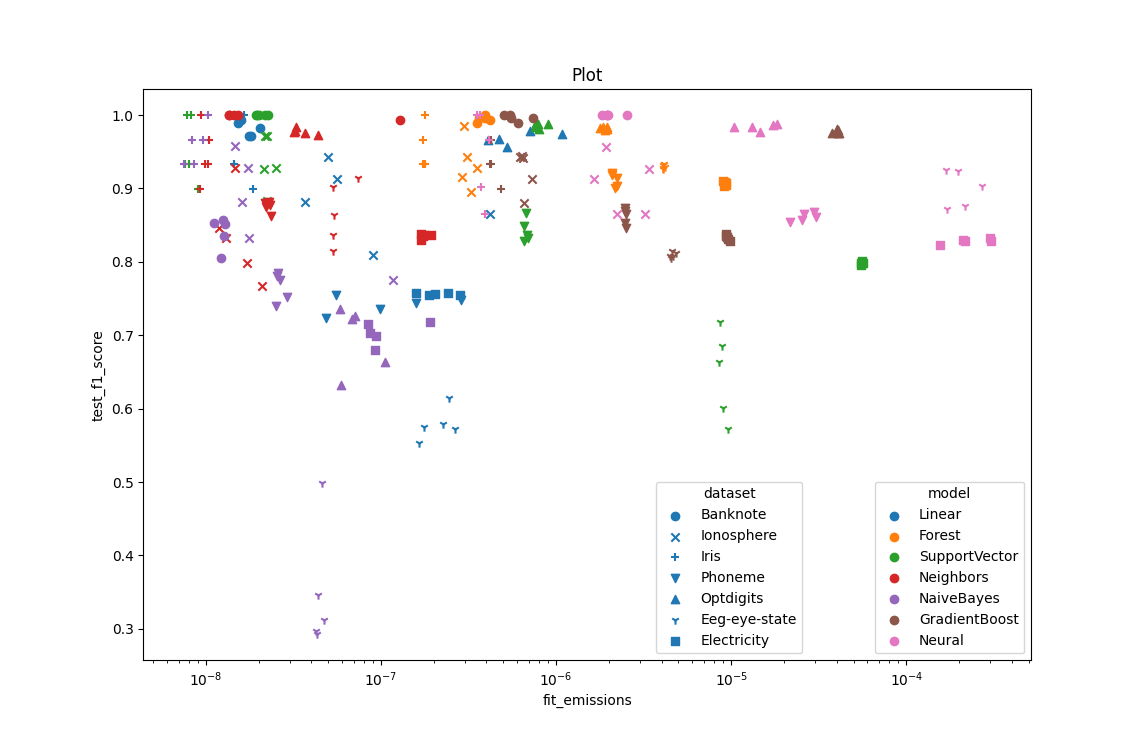
\includegraphics[width=1.3\textwidth, keepaspectratio]{img/graph/4scatter-dataset-model.png}
  }
  \caption{Valor-F alcanzado por el modelo frente a las emisiones de carbono necesarias para entrenarlo, por modelo empleado y conjunto de datos utilizado}
  \label{fig:scatter-1}
\end{figure}
\todo[inline]{Fix plot titles}

\todoin{Desarrollo explicación scatter plot:\\
> Outlier eeg-eye-state lower score, high variance \\
> Neural, higher emissions, average score, high variance, better score more complex dataset  \\
> Support vector, starts well, but low score for eye and very high emissions for electricity \\

> Forest, high score, medium emissions, even for eye dataset  \\
> Gradient, same but a little worse on both \\

> Neighbors, very low emissions \\

> Linear, low emissions, low score \\
> Naive bayes, very low score, low emissions \\ \\ \\
Marcar areas en la gráfica siguiendo la discusión para mejor visualización ? \\
}


\begin{figure}[H]
  \centerline{
     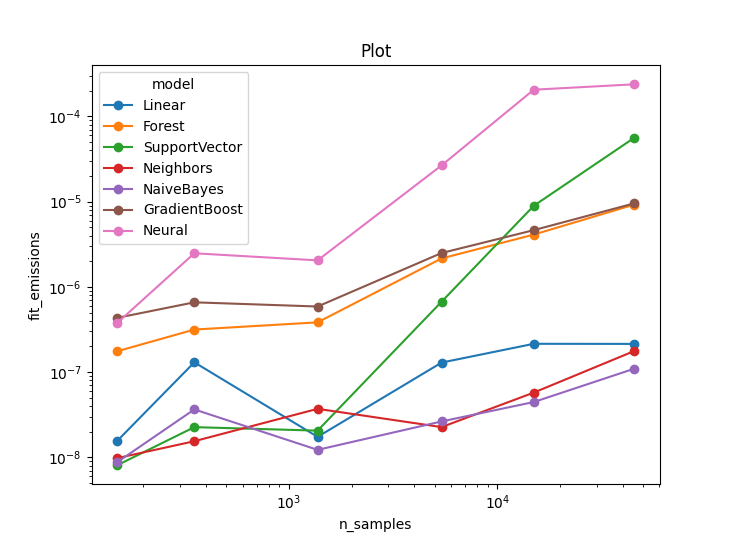
\includegraphics[width=1\textwidth, keepaspectratio]{img/graph/line-nsamples-emission-log.png}
  }
  \caption{Evolución de las emisiones de carbono con el aumento de número de muestras del conjunto de datos}
  \label{fig:line-emissions-samples}
\end{figure}
\begin{figure}[H]
  \centerline{
     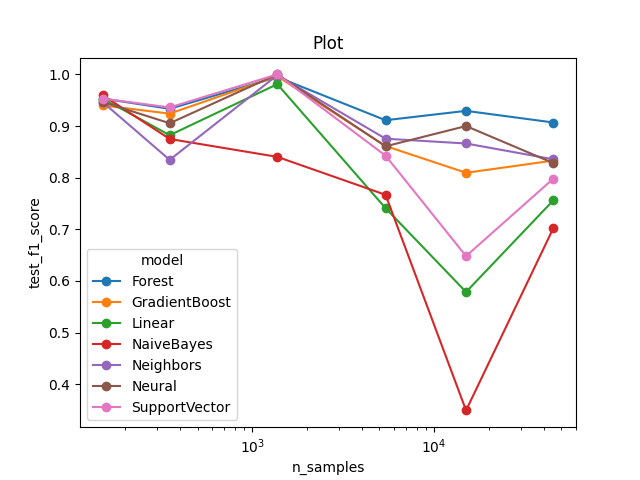
\includegraphics[width=1\textwidth, keepaspectratio]{img/graph/line-nsamples-fscore-loglin.png}
  }
  \caption{Evolución de las emisiones de carbono con el aumento de número de muestras del conjunto de datos}
  \label{fig:line-fscore-samples}
\end{figure}

\todoin{Line plots: \\
> Mejores puntuaciones: Forest, Neural, Neighbors \\
> Producen emisiones: media, alta, baja, respectivamente \\
}


\section{Consumo energético en función de los recursos disponibles}
\label{sec:test-2-resources}

\subsubsection{Objetivos}

 En el experimento anterior se observó que el modelo utilizado en el entrenamiento determina en gran medida el consumo energético. Sin embargo, hay una dimensión más que se puede estudiar para intentar reducir este consumo: los recursos computacionales dedicados a la tarea. Al utilizar un ordenador con menores recursos, el proceso de entrenamiento sin duda llevará más tiempo que en una máquina con mayores recursos. Sin embargo, su consumo energético por unidad de tiempo será comparativamente menor.
 
 En esta sección pretende analizar que configuración de recursos actuará de forma más eficiente durante el entrenamiento de un conjunto de datos de gran tamaño, atendiendo a las siguientes cuestiones:

 \begin{itemize}
    \item Si es posible compensar más tiempo con menos consumo.
    \item Si se puede encontrar alguna combinación de recursos especialmente eficiente.
    \item Como afectan los recursos empleados a la calidad de las predicciones.
\end{itemize}

\subsubsection{Metodología}

La característica principal a analizar de las máquinas utilizadas será el número de procesadores dedicados a las tareas de entrenamiento. En un ordenador de un solo núcleo, cada iteración de la validación cruzada debe realizarse secuencialmente. Sin embargo, al aumentar el número de núcleos del procesador, es posible realizar las tareas de forma paralela. Para utilizar este mecanismo, es necesario activarla indicando a \texttt{scikit-learn} la opción \texttt{n\_jobs=-1} para indicar el número de procesos a ejecutar en paralelo, donde -1 indica utilizar todos los disponibles.

Para analizar como afecta el número de procesadores disponibles al consumo energético, se tomarán medidas en máquinas con tres configuraciones diferentes. Estas máquinas serán desplegadas como máquinas virtuales en la nube, lo que facilitará controlar los recursos disponibles para cada configuración y ofrecerá un entorno similar de trabajo para todos los casos. La plataforma elegida para el despliegue es Microsoft Azure (sección~\ref{subsec:azure}), que ofrece una gran capacidad de personalización en los recursos desplegados y cuenta con una oferta de créditos gratuitos para el sector educativo que pueden ser empleados en minutos de ejecución de maquinas virtuales.

El proceso seguido será similar para cada combinación de recursos elegida. En primer lugar es necesario desplegar la máquina virtual con una red virtual configurada que permita conexiones mediante \texttt{ssh}, para poder ser controlada por línea de comandos. A continuación, se ejecutará el script \texttt{azure/install.sh} ubicado en el repositorio del proyecto\footnote{\url{https://github.com/l-gonz/tfg-gitt-mlcost/blob/main/azure/install.sh}}. Este script instalará la aplicación MLCost y todas sus dependencias, tomará una serie de medidas de entrenamiento en un conjunto de datos concreto, y exportará los resultados para su posterior análisis.

El conjunto de datos elegido para analizar este proceso será \emph{electricity} (ver \ref{subsec:dataset-electricity}), que contiene alrededor de 45K muestras. Este tamaño moderado permite ejecutar los experimentos en un tiempo razonable del orden de pocos minutos por modelo. Al mismo tiempo, tiene un tamaño suficiente para que las diferencias de consumo generadas por las distintas configuraciones de recursos sean visibles.
Las configuraciones de recursos elegidas para las máquinas virtuales están recogidas en la Tabla~\ref{tab:caracteristicas-tecnicas-multi}. El Anexo \ref{ax:az-templates} contiene unas plantillas que se pueden utilizar dentro de Microsoft Azure para desplegar máquinas virtuales con una configuración idéntica a las utilizadas para tomar las medidas de este experimento.
\todo[inline]{Guardar plantillas}

El proceso completo seguido para cada configuración de recursos puede resumirse en los siguientes pasos:
\begin{enumerate}
    \item Desplegar una máquina virtual en la nube con la configuración deseada.
    \item Conectarse a la máquina virtual mediante SSH.
    \item Descargar el repositorio del proyecto.
    \item Ejecutar el script \texttt{azure/install.sh}.
\end{enumerate}


\begin{table}[h]
    \caption{Características técnicas de las máquina virtuales comparadas}
    \label{tab:caracteristicas-tecnicas-multi}
    \renewcommand\arraystretch{1.6}
    \centering
    \begin{tabular}{>{\raggedright\arraybackslash}m{0.2\textwidth}
                    >{\centering\arraybackslash}m{0.2\textwidth}
                    >{\centering\arraybackslash}m{0.2\textwidth}
                    >{\centering\arraybackslash}m{0.2\textwidth}
                    }
    \toprule
    \textbf{Característica}  
    & \textbf{Test 1}                             
    & \textbf{Test 2}                             
    & \textbf{Test 3} \\ \midrule
Sistema operativo     
    & \multicolumn{3}{c}{Ubuntu 20.04.6 LTS x86\_64} \\
Procesador            
    & \multicolumn{3}{c}{\begin{tabular}[c]{@{}c@{}}Intel(R) Xeon(R) Platinum 8272CL CPU @ 2.60GHz\end{tabular}} 
     \\
Versión Python                
    & \multicolumn{3}{c}{3.12.3}  \\
Configuración Azure               
    & B1s   & B2ms   & B4ms  \\
Memoria (GB)              
    & 0,8?   & 7,75  & 15,57  \\
vCPUs 
    & 1   & 2   & 4  \\
    \bottomrule
\end{tabular}
\end{table}

% Low - B1s: 1vcpu, 1GB ram

% Mid - B2ms: 2vcpus, 8GB ram

% Xtra - B4ms: 4vcpus, 16GB memory
% Running on paralleltest3
% Intel(R) Xeon(R) CPU E5-2673 v4 @ 2.30GHz
% Memory: 15.57 GB
% Start load: 4.00% for 4 CPUs


\subsubsection{Resultados}

\begin{figure}[H]
  \centerline{
     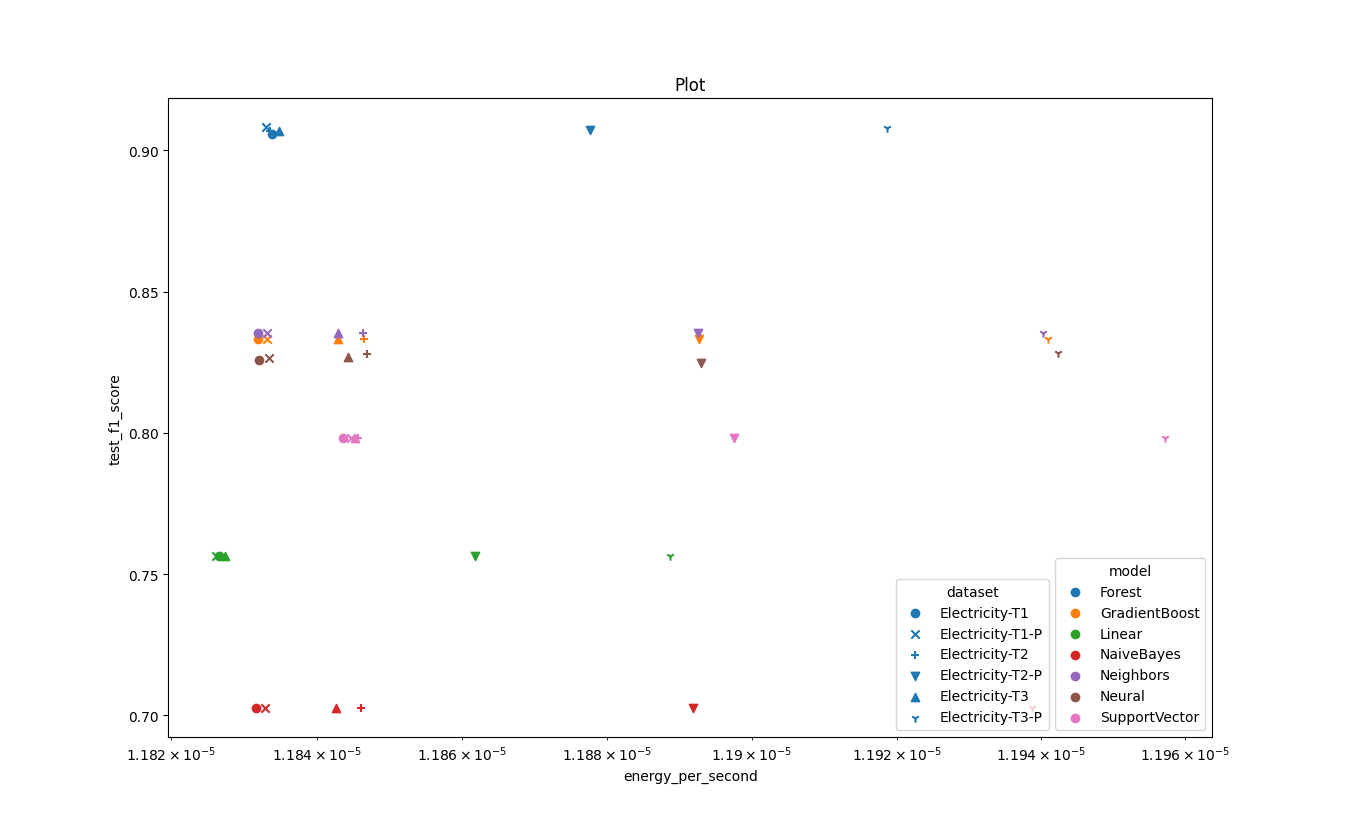
\includegraphics[width=\textwidth, keepaspectratio]{img/graph/2-scat-energy-p-s.png}
  }
  \caption{Distribución de la energía por segundo}
  \label{fig:4-2-energy-per-second}
\end{figure}
\begin{figure}[H]
  \centerline{
     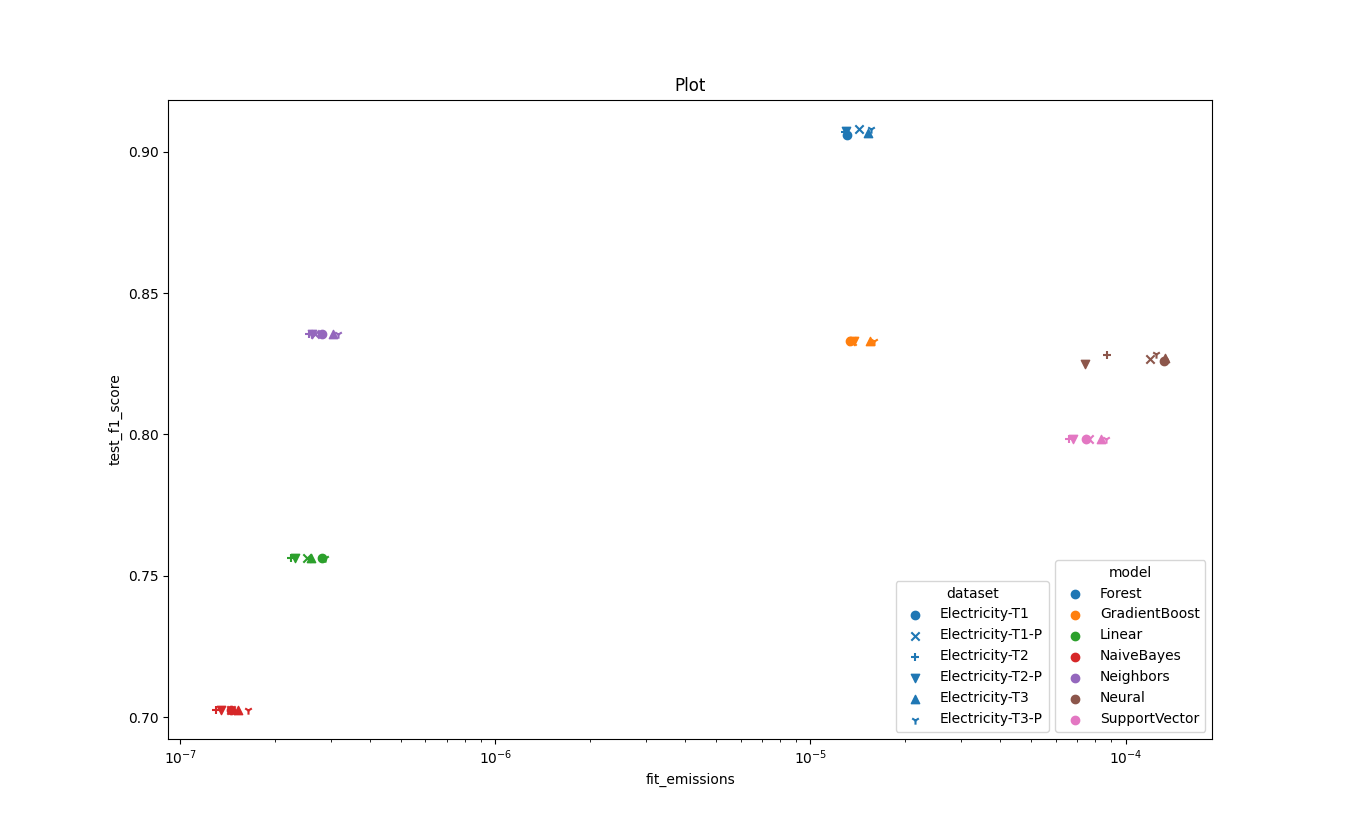
\includegraphics[width=\textwidth, keepaspectratio]{img/graph/2-scat-fit-emissions.png}
  }
  \caption{Distribución de las emisiones por hilo de ejecución}
  \label{fig:4-2-energy-per-second}
\end{figure}
\begin{figure}[H]
  \centerline{
     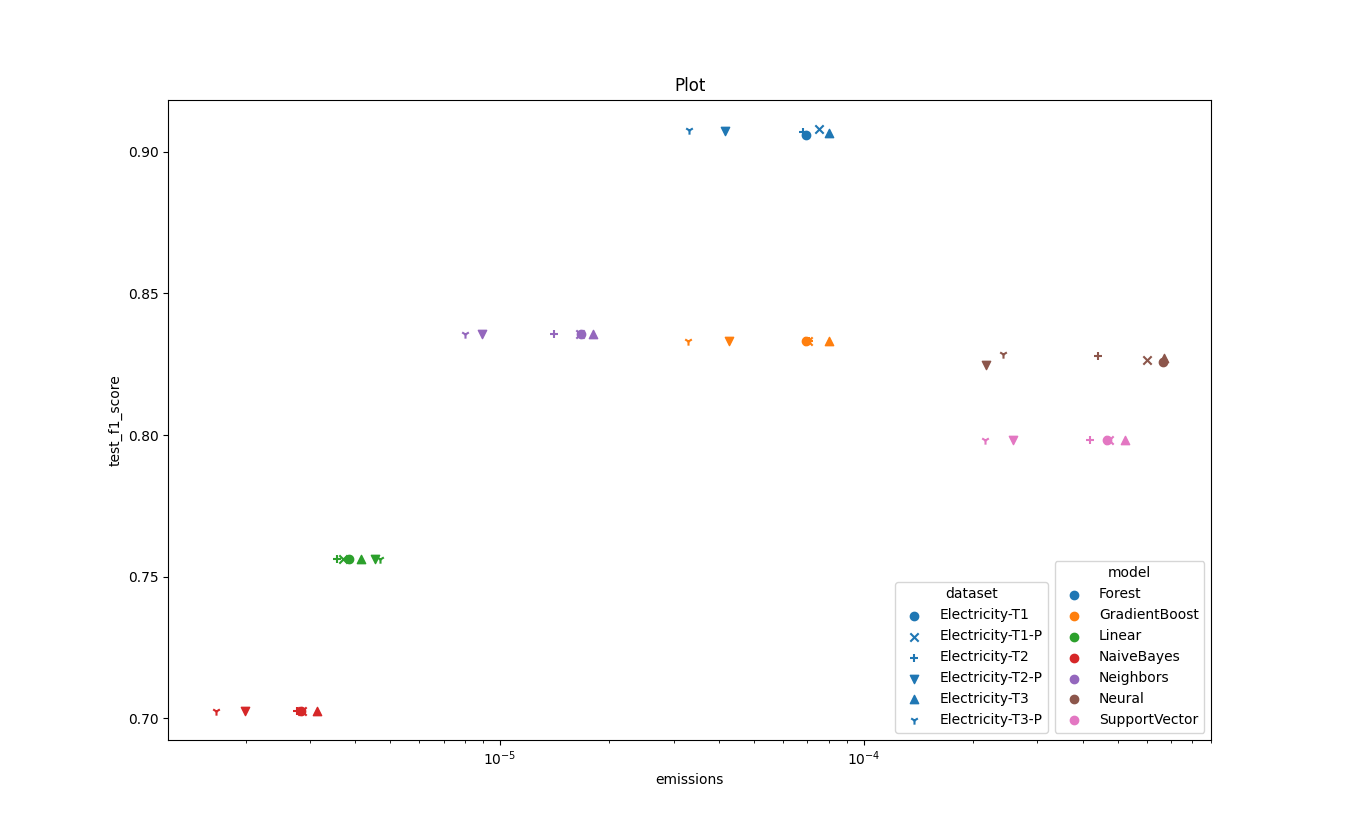
\includegraphics[width=\textwidth, keepaspectratio]{img/graph/2-scat-emissions.png}
  }
  \caption{Distribución de las emisiones totales del entrenamiento}
  \label{fig:4-2-energy-per-second}
\end{figure}

\todoin{Análisis: \\
> Dice algo f\_score en el eje y? Cambiar? \\
> Energía por segundo es la misma prácticamente para todos los casos \\
> En emisiones totales sí consume menos las opciones -P (excepto T1, por tener solo 1 procesador es lo mismo) (excepto Linear model, no paraleliza ??)
> En emisiones por iteración no hay apenas diferencia (T2 consume menos en general por poco) \\ \\ 

> ¿Cambiar y tomar medidas con -cv 8 para ser divisible entre número cpus de todas las configuraciones?
}

% \section{?? Optimización del consumo energético}

% \todoin{Proceso: \\
% > Elegir 2-3 modelos interesantes \\
% > Run GridSearchCV \\
% > Optimizar hiperparámetros para reducir consumo \\
% > Cambia que modelos son más eficientes con la optimización ???
% }

% \section{?? Consumo energético en función de la localización}

% \todoin{
% > codecarbon permite indicar el país al medir el consumo \\
% > el calculo de energía a kg CO2 equivalentes cambia mucho \\
% > codecarbon-viz tool tiene gráficas de como varía el consumo por país, como se compara el consumo a usos domésticos
% }

\clearpage